\documentclass[t]{beamer}
% \includeonlyframes{cm20}

\usepackage[utf8x]{inputenc}
\usepackage[ngerman]{babel}
\usepackage[T1]{fontenc}
\usepackage{textcomp}
\usepackage{subfigure}
\usepackage{graphicx}
\usepackage{fancyhdr}
\usepackage{tgpagella}
\usepackage[absolute,overlay]{textpos}
\usepackage{hyperref}
\usepackage{wasysym}
\usepackage{color}
\usepackage{tcolorbox}
\usepackage{tikz}

% ohne dieses Paket bekommt Carsten verpixelte Schrifen
\usepackage{lmodern}

\usetikzlibrary{decorations.pathreplacing}
\usetikzlibrary{calc}



\hypersetup{
colorlinks=true,
linkcolor=[rgb]{1, 1, 1}, %
urlcolor=[rgb]{.2, .2, .5} %
%allcolors=[rgb]{0, 0, 0} % schwarz
}

\usetheme{Dresden}
\useoutertheme{infolines}

% \setbeamerfont*{quote}{family=\sffamily}
% \addtobeamertemplate{quote begin}{}{\begin{tcolorbox}}
% \addtobeamertemplate{quote end}{\end{tcolorbox}}{}

\setbeamertemplate{navigation symbols}{} % we dont want navigation buttons

\title{Freie Software Freies Wissen Dresden}
\subtitle{Fund-Raising for Free Software - Thinking Big}
\author{\texttt{https://fsfw-dresden.de}}
\date{2018-12-29 (35C3)}



\addtobeamertemplate{frametitle}{}{%
  \begin{textblock*}{130mm}(.87\textwidth,8.4mm)
    
\includegraphics[width=2.25cm]{img-src/fsfw-logo.pdf}
  \end{textblock*}
}


\setbeamercolor{frametitle}{fg=black}

\synctex=1


\definecolor{softblue}{rgb}{0.3,0.3,.6}
\definecolor{lightblue}{rgb}{0.9,0.9,.95}
\newenvironment{cboxed}[1]
{\begin{tcolorbox}[colback=lightblue,colframe=softblue,title=#1]}
{\end{tcolorbox}}
\newenvironment{bboxed}
{\begin{tcolorbox}[colback=lightblue,colframe=softblue]}
{\end{tcolorbox}}

\newcommand{\cst}[1]{{\usebeamercolor[fg]{structure}#1}}




\begin{document}

\begin{frame}[label=p1]
  \begin{center}%
\vspace*{-1em}

\includegraphics[width=4cm]{img-src/fsfw-logo-with-text}
% \hspace{1cm}
% \includegraphics[width=4cm]{img-src/gutschein-seite-1}\\
\vspace{-1em}

\begin{minipage}{37mm}
\begin{center}
Hochschulgruppe für\\
Freie Software und\\
Freies Wissen Dresden
\end{center}
\end{minipage}
\end{center}


\vspace{2em}
\hfill \structure{\LARGE "`Fund-Raising for Free Software - Thinking Big"'}
\vspace{1em}

\hfill \footnotesize{(Carsten Knoll)}~~
\end{frame}

%%%%%%%%%%%%%%%%%%%%%%%%%%%%%%%%%%%%%%%%%%%%%%%%%%%%%%%%%%%%%%%%%%%%%%%%%%%%%%%%

\begin{frame}[label=ol]{\usebeamercolor[fg]{structure}\color{fg}Overview}
  \begin{itemize}
  \setlength\itemsep{1em}
  \item Who we are and what we do
  \item Theses about free software for desktop usage
  \item Analysis of existing business models
  \item Idea: Combination-Model -- Selling Support Certificates
  \item How to proceed? $\rightarrow$ Discussion
  \end{itemize}
\end{frame}




%%%%%%%%%%%%%%%%%%%%%%%%%%%%%%%%%%%%%%%%%%%%%%%%%%%%%%%%%%%%%%%%%%%%%%%%%%%%%%%%

\begin{frame}[label=ct1]{\usebeamercolor[fg]{structure}\color{fg}FSFW: Who are we?}

  \begin{itemize}
  \item University group for Free Software and Free Knowledge {\footnotesize (founded 2014)}
  \item Projects:
  \begin{itemize}
   \item Linux-Install-Party, Linux-Presentation-Day
   \item Encryption competition
   \item Monthly \href{https://fsfw-dresden.de/sprechstunde}{Help desk} (\LaTeX, Libre-Office, ...)
   \item Publications: \href{https://fsfw-dresden.de/programm}{Programmpapier}, \href{https://fsfw-dresden.de/blog}{Blogposts}
   \item Workshops (\href{https://fsfw-dresden.de/git-ws}{git}, \href{https://fsfw-dresden.de/python-workshop}{python},
   \href{https://fsfw-dresden.de/gpg}{EMail encryption})
   \item Weekly lecture (Ringvorlesung): \\
   "`\href{https://fsfw-dresden.de/ringvorlesung}{Free Software and Free Knowledge as Profession}"'
   \smallskip
   \item UniStick: 8GB with useful\\
   Free Software for university students
  \end{itemize}
  \end{itemize}


% \begin{textblock*}{40mm}[0.,0.](90mm,32mm)
\begin{textblock*}{40mm}[0.,0.](25mm,70mm)
  \visible<2->{
    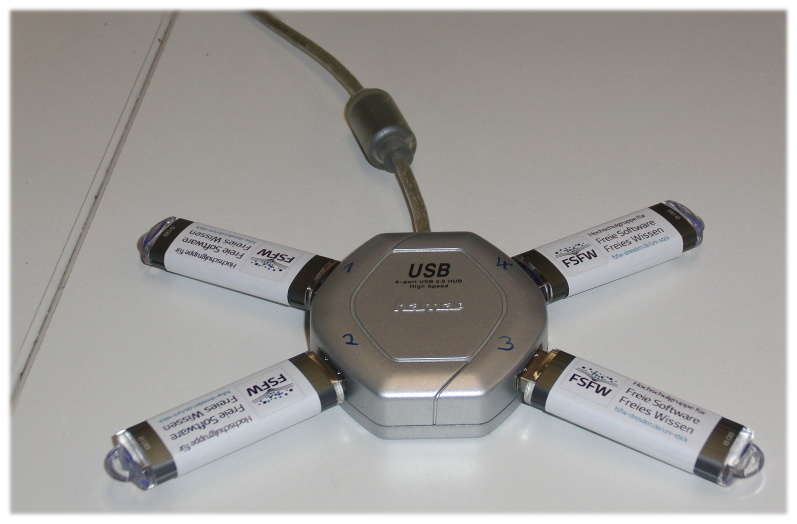
\includegraphics[width=30mm]{img-src/usb-hub}
  }
\end{textblock*}

\begin{textblock*}{55mm}[0.,0.](80mm,60mm)
  \visible<3->{
    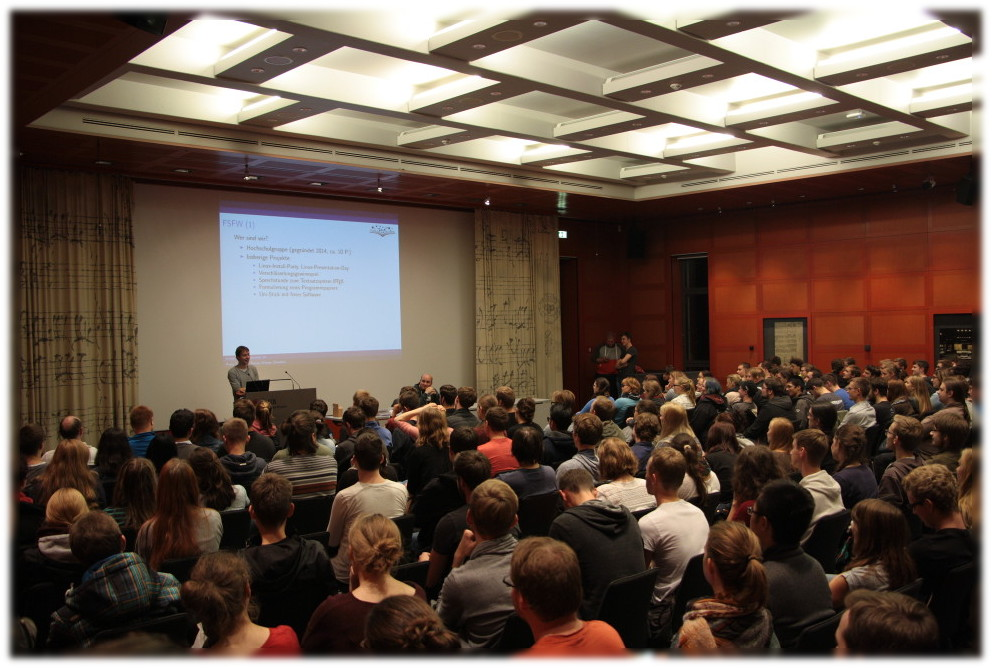
\includegraphics[width=45mm]{img-src/uni-stick-ausgabe-vortrag}
  }
\end{textblock*}

\end{frame}

%%%%%%%%%%%%%%%%%%%%%%%%%%%%%%%%%%%%%%%%%%%%%%%%%%%%%%%%%%%%%%%%%%%%%%%%%%%%%%%%

\begin{frame}[label=ct2]{\usebeamercolor[fg]{structure}\color{fg}FSFW: Why do we do this?}
 $\rightarrow$ \textbf{By  Conviction}\\[1cm]
  \begin{itemize}
  \item \textbf{Conviction 1}:\\
  Free and Open Source Software is (mostly) the better choice
  \item[] (technical/non-technical Arguments).
  \pause
  \bigskip
  \item \textbf{Conviction 2}:\\
  Scientific contents \textit{financed with public money}
  (authors, reviewers) should not be sold to \textit{public}
  libraries for \textit{ridiculous prices} by journal publishers.
  \end{itemize}
\end{frame}

%%%%%%%%%%%%%%%%%%%%%%%%%%%%%%%%%%%%%%%%%%%%%%%%%%%%%%%%%%%%%%%%%%%%%%%%%%%%%%%%


\begin{frame}[label=ct3,plain]{}

\vspace{1mm}
\begin{center}
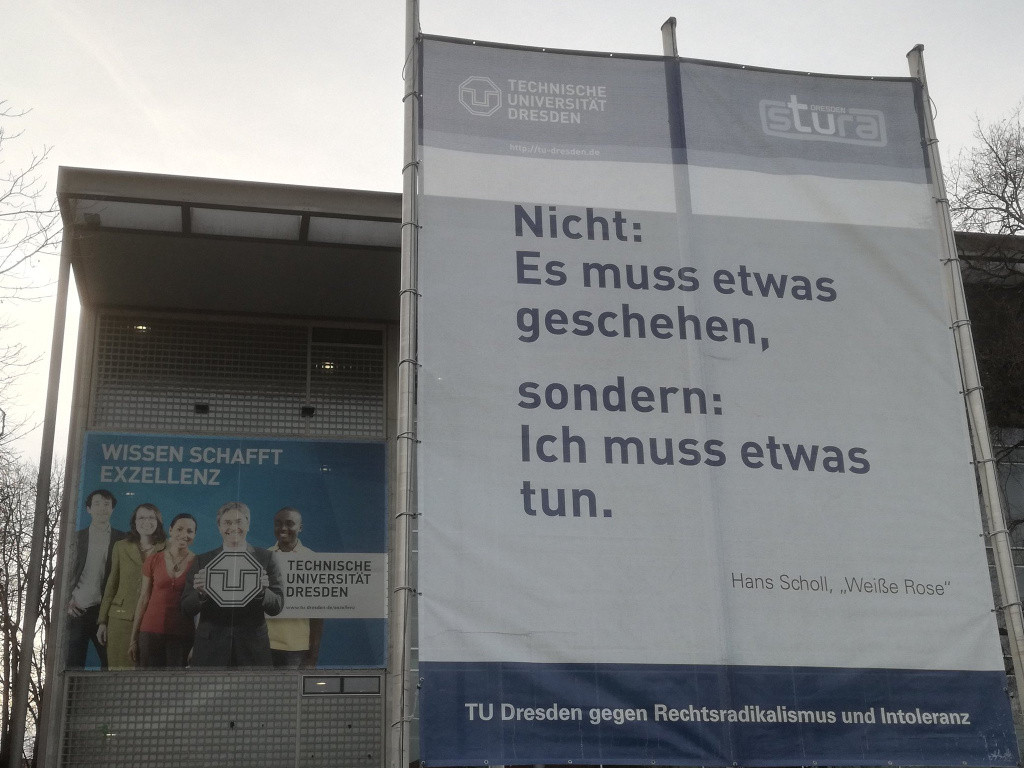
\includegraphics[width=1.05\textwidth]{img-src/tud-ich-muss-etwas-tun}
\end{center}
\only<2->{
\begin{textblock*}{0.55\textwidth}[0.,0.](55mm,28mm)
\begin{bboxed}
\visible<2>{
\Large
\vspace{3mm}
Not:\\
``Somthing has to happen!''
\vspace{7mm}

But instead:\\
``I have to do something!''
}
\end{bboxed}
\end{textblock*}

\begin{textblock*}{0.55\textwidth}[0.,0.](58mm,48mm)
\visible<3->{

\includegraphics[width=0.9\textwidth]{img-src/tuwat_logo}
}
\end{textblock*}

}

\end{frame}
%%%%%%%%%%%%%%%%%%%%%%%%%%%%%%%%%%%%%%%%%%%%%%%%%%%%%%%%%%%%%%%%%%%%%%%%%%%%%%%%


\begin{frame}[label=ct4,plain]{}

\vspace{1mm}
\begin{center}
\href{https://fsfw-dresden.de/fork}{
\includegraphics[width=1.0\textwidth]{img-src/fsfw-fork.pdf}}
\end{center}


\end{frame}
%%%%%%%%%%%%%%%%%%%%%%%%%%%%%%%%%%%%%%%%%%%%%%%%%%%%%%%%%%%%%%%%%%%%%%%%%%%%%%%%


\begin{frame}[label=ct5]{}

\begin{center}
\textbf{Following thoughts are also available as a blogpost:}

\vspace{10mm}

\structure{\LARGE \url{https://fsfw-dresden.de/funding-foss}}
\vspace{10mm}


\includegraphics[width=0.3\textwidth]{img-src/qr-code-funding-foss.png}

\end{center}
\end{frame}

%%%%%%%%%%%%%%%%%%%%%%%%%%%%%%%%%%%%%%%%%%%%%%%%%%%%%%%%%%%%%%%%%%%%%%%%%%%%%%%%
% content
%%%%%%%%%%%%%%%%%%%%%%%%%%%%%%%%%%%%%%%%%%%%%%%%%%%%%%%%%%%%%%%%%%%%%%%%%%%%%%%%
\newlength{\breite}


\begin{frame}[label=obs1]{\usebeamercolor[fg]{structure}Theses about Free Software for Desktop Usage}
\begin{enumerate}
\item There exist amazing products.
\pause
\medskip

\item Society would benefit from higher FOSS market share.
\pause
\medskip

\item FOSS has only a small market share.
\pause
\medskip

\item Many projects suffer from lacking resources,\\
user experience could be better with more resources.
\pause
\bigskip
\bigskip

\item
\end{enumerate}


\begin{textblock*}{\textwidth}[0.,0.](10mm,55mm)
\setlength{\breite}{0.9\textwidth}
\only<+>{\includegraphics[width=\breite]{img-src/ffi_feedback_loop-01}}
\only<+>{\includegraphics[width=\breite]{img-src/ffi_feedback_loop-02}}

\end{textblock*}


\end{frame}

%%%%%%%%%%%%%%%%%%%%%%%%%%%%%%%%%%%%%%%%%%%%%%%%%%%%%%%%%%%%%%%%%%%%%%%%%%%%%%%%

\begin{frame}[label=obs2]{\usebeamercolor[fg]{structure}Observations}
Widespread ``classical'' business model:
\begin{itemize}
 \item Selling software usage rights or collected data
 \item Use revenues for development and PR
\end{itemize}
\pause
\smallskip
Not possible nor desired for FOSS

\pause
\medskip

{\usebeamercolor[fg]{structure}Why does the concept of ``Free Software'' work at all?}

\bigskip
People dedicate time and effort to FOSS-projects
\begin{itemize}
 \item driven by enthusiasm
 \item for fun
 \item to show their skills
 \item to learn new skills
 \bigskip

 \pause
 \item for money (raised by some exsiting FOSS business model)
\end{itemize}


\end{frame}

%%%%%%%%%%%%%%%%%%%%%%%%%%%%%%%%%%%%%%%%%%%%%%%%%%%%%%%%%%%%%%%%%%%%%%%%%%%%%%%%
%%%%%%%%%%%%%%%%%%%%%%%%%%%%%%%%%%%%%%%%%%%%%%%%%%%%%%%%%%%%%%%%%%%%%%%%%%%%%%%%

\begin{frame}[label=ol30]{}

\vspace{0.3\textheight}
\LARGE
\begin{center}
 \usebeamercolor[fg]{structure} Analysis of Existing FOSS Business Models
\end{center}

\end{frame}

%%%%%%%%%%%%%%%%%%%%%%%%%%%%%%%%%%%%%%%%%%%%%%%%%%%%%%%%%%%%%%%%%%%%%%%%%%%%%%%%

\begin{frame}[label=obs3]{\usebeamercolor[fg]{structure}Existing FOSS Business Models}

Wikipedia: \href{https://en.wikipedia.org/wiki/Business_models_for_open-source_software}{18 business models}

\pause
\medskip
Not applicable/desired for sustainable end-user software:
\begin{itemize}
 \item Open sourcing on end-of-life,  dual-licensing, ...
 \pause
 \item Selling support,  delayed open-sourcing, proprietary extensions
\end{itemize}
\pause

Remainder:

\begin{enumerate}
\item Selling of branded merchandise
\item Selling of certificates and trademark use
\item Partnership with funding organizations
\item Bounty driven development
\item Crowdfunding/reverse-bounty model
\item Advertising-supported software
\item Voluntary donations
\end{enumerate}


\end{frame}

%%%%%%%%%%%%%%%%%%%%%%%%%%%%%%%%%%%%%%%%%%%%%%%%%%%%%%%%%%%%%%%%%%%%%%%%%%%%%%%%

\begin{frame}[label=obs4]{\usebeamercolor[fg]{structure}``Voluntary Donations''}

\begin{itemize}
 \item Contradict \textit{economic rationality}?
 \tikz[remember picture] \node[coordinate,yshift=0.7em] (A) {};

 \item Express irrational altruism?
 \tikz[remember picture] \node[coordinate, xshift=9mm] (B) {};
\end{itemize}

\visible<2->{
\begin{tikzpicture}[overlay,remember picture]

  \draw[thick,decorate,decoration={brace,amplitude=5pt}]
        (A-|B) -- (B) node[midway, right=4pt] {\hspace{-1mm} No! {\footnotesize (For a sane definition of rationality)}};
\end{tikzpicture}
 } % end visible

\pause
\pause
\begin{cboxed}{Subjective Sidenote}
Model of \href{https://en.wikipedia.org/wiki/Homo_economicus}{homo economicus}
describes an extremely shortsighted psychopathic personality.
Much of the worlds problems originate in mistakenly propagating it as \textit{normative} role model.
\end{cboxed}

\pause
Established examples of ``irrational spending''
\begin{itemize}
 \item Brand awareness and status consumption\\
 \item Future-oriented self-interest
\end{itemize}

\end{frame}

%%%%%%%%%%%%%%%%%%%%%%%%%%%%%%%%%%%%%%%%%%%%%%%%%%%%%%%%%%%%%%%%%%%%%%%%%%%%%%%%
%%%%%%%%%%%%%%%%%%%%%%%%%%%%%%%%%%%%%%%%%%%%%%%%%%%%%%%%%%%%%%%%%%%%%%%%%%%%%%%%

\begin{frame}[label=ol40]{}

\vspace{0.3\textheight}
\LARGE
\begin{center}
 \usebeamercolor[fg]{structure} Combination Model
\end{center}

\end{frame}

%%%%%%%%%%%%%%%%%%%%%%%%%%%%%%%%%%%%%%%%%%%%%%%%%%%%%%%%%%%%%%%%%%%%%%%%%%%%%%%%


\begin{frame}[label=cm10]{\cst{Combination Model (Overview)}}
\begin{textblock*}{\textwidth}[0.,0.](10mm,20mm)
\setlength{\breite}{0.9\textwidth}
\only<+>{\includegraphics[width=\breite]{img-src/ffi_principle-01}}
\only<+>{\includegraphics[width=\breite]{img-src/ffi_principle-02}}
\only<+>{\includegraphics[width=\breite]{img-src/ffi_principle-03}}
\only<+>{\includegraphics[width=\breite]{img-src/ffi_principle-04}}
\only<+>{\includegraphics[width=\breite]{img-src/ffi_principle-05}}
\only<+>{\includegraphics[width=\breite]{img-src/ffi_principle-06}}
\only<+>{\includegraphics[width=\breite]{img-src/ffi_principle-07}}
\only<+>{\includegraphics[width=\breite]{img-src/ffi_principle-08}}
\only<+>{\includegraphics[width=\breite]{img-src/ffi_principle-09}}
\bigskip
\only<1-5>{
\begin{itemize}
 \item<1-2> Challenge: several users want to fund several projects
 \item<3> Current situation: $n$-to-$m$ relationship $\rightarrow$ bad effort-benefit ratio
 \item<4-5> Proposal: specialized organization\\
 Working title: ``Funding Freedom Initiative'' (FFI)
\end{itemize}
}
\only<6-8>{
\begin{itemize}
 \item<6-8> Users \textit{buy} ``Free Software Support Certificates'' {\footnotesize for  e.\,g. 0.1 EUR/day}\\
\visible<7-8>{  (and optionally get high quality merchandise material) }
 \item<8> Users (optionally) state their preferred projects\\
 $\rightarrow$ Funds can be distributed accordingly
\end{itemize}
}
\only<9->{
\begin{itemize}
 \item<9> Interested projects register once and\\
 regularly publish activity reports
\end{itemize}
}

\end{textblock*}

\end{frame}


%%%%%%%%%%%%%%%%%%%%%%%%%%%%%%%%%%%%%%%%%%%%%%%%%%%%%%%%%%%%%%%%%%%%%%%%%%%%%%%%


\begin{frame}[label=cm20]{\cst{Why should people spend money on this?}}
\vspace{10mm}
% {\large \textbf{Why should people spend money on this?}}
% \vspace{5mm}

\pause

\begin{enumerate}
\setlength\itemsep{2em}
 \item<+->  Support for Free Software ($\rightarrow$ \textit{Voluntary donation})

\only<3>{
\vspace{10mm}
% \begin{center}
Role model: \hspace{7mm}
\raisebox{-15mm}{ 
\includegraphics[width=0.6\textwidth]{img-src/atmosfair_logo_en}}
% \end{center}

}
\pause
 \item<+->  Merchandise material ($\rightarrow$ \textit{Selling of branded merchandise})\\
 \only<5>{
\vspace{3mm}
 \begin{bboxed}
\Large
\vspace{5mm}
Imagine picture of 35C3 t-shirt queue here.
\vspace{7mm}
\end{bboxed}
}
\pause
 \item<+->  (Maybe) Privileged communication channel into the project team\\
 ($\rightarrow$ \textit{Bounty Driven Development}; $\rightarrow$ \textit{Selling support})
 \item<+-> (Maybe) Extra-features/no ads ($\rightarrow$ \textit{Advertising supported software})\\[1mm]
%  \pause
\visible<+->{
 {\footnotesize \hfill (Might be controversial $\rightarrow$ up to discussion)}
}
\end{enumerate}

\end{frame}

%%%%%%%%%%%%%%%%%%%%%%%%%%%%%%%%%%%%%%%%%%%%%%%%%%%%%%%%%%%%%%%%%%%%%%%%%%%%%%%%
\begin{frame}[label=cm30]{\cst{How could the money be distributed?}}
\vspace{2mm}
% {\large \textbf{How could the money be distributed?}}

\pause
\begin{textblock*}{\textwidth}[0.,0.](05mm,25mm)
\hspace{10mm}
\setlength{\breite}{0.9\textwidth}
\only<+>{\includegraphics[width=\breite]{img-src/ffi_principle-10}}
\only<+>{\includegraphics[width=\breite]{img-src/ffi_principle-11}}
\only<+>{\includegraphics[width=\breite]{img-src/ffi_principle-12}}
\only<+>{\includegraphics[width=\breite]{img-src/ffi_principle-13}}
\only<+>{\includegraphics[width=\breite]{img-src/ffi_principle-14}}

\smallskip
\only<2->{
\textbf{Split certificate price into categories (C1--C4)}
\vspace{-2mm}
\begin{columns}
\column[t]{0.5\textwidth}
\begin{itemize}
 \item<3-> C1 (e.\,g. 70\%): distribute \\
  according to user preferences
 \item<4-> C2 (e.\,g. 20\%):\\
 use for strategic support
\end{itemize}
\column[t]{0.5\textwidth}
\begin{itemize}
 \item<5-> C3 (e.\,g. 10\%):\\
 FFI operating cost
 \item<6-> C4 (extra):\\
 material cost (merchandise)
\end{itemize}
\end{columns}

}
\end{textblock*}


\end{frame}

%%%%%%%%%%%%%%%%%%%%%%%%%%%%%%%%%%%%%%%%%%%%%%%%%%%%%%%%%%%%%%%%%%%%%%%%%%%%%%%%
\begin{frame}[label=cm40]{\cst{How can embezzlement be prevented?}}
\vspace{10mm}
% {\large \textbf{How can embezzlement be prevented?} }

\begin{itemize}
\setlength\itemsep{2em}
 \item Complete transparency of money streams
 \item Combined with data frugality and respect for users privacy
\end{itemize}
\pause
\vspace{10mm}
\begin{center}
\textbf{$\rightarrow$ More details: see \href{https://fsfw-dresden.de/2018/11/funding-foss-en.html\#criticism}{blog post}}
\end{center}

\end{frame}

%%%%%%%%%%%%%%%%%%%%%%%%%%%%%%%%%%%%%%%%%%%%%%%%%%%%%%%%%%%%%%%%%%%%%%%%%%%%%%%%
\begin{frame}[label=cm50]{\cst{What happens with the money ?}}
Projects can
\begin{itemize}
 \item get the money paid off (+ take care of taxation)
 \item pass it to other projects (e.\,g. libs on which they depend)
\end{itemize}

\pause
\textbf{Excerpts from imaginary activity reports:}
\only<2-4>{
\begin{itemize}
 \item<+-> \textit{``Could afford to reduce my weekly working hours and spend more time on Project XYZ.''}
 \item<+-> \textit{``The money was used to pay for an ad campaign (print and online). The download numbers have tripled in that period. We would like to do that again.''}
 \item<+-> \textit{``Thanks to the money we were able to integrate two employees from our usability team to the project, each with 20\% full time. Additionally, a student assistant has updated the documentary.''}
\end{itemize}
}
\only<5->{
\begin{itemize}
 \item<5-> \textit{``We have contracted company XYZ to fix Issue 123. For the future we plan the same with issue 456.''}
\item<6-> \textit{``I see the money as recognition for the work done in the last year. Thanks guys!''} (Similar to the Bounty model)
\item<7-> \textit{``In the last quarter, issues were mainly addressed that were highly valued by donors. Details: see release notes.''} (reverse bounty model)


\end{itemize}

}




\end{frame}

%%%%%%%%%%%%%%%%%%%%%%%%%%%%%%%%%%%%%%%%%%%%%%%%%%%%%%%%%%%%%%%%%%%%%%%%%%%%%%%%
\begin{frame}[label=cm70]{\cst{Potential points of criticisms}}
\begin{itemize}
 \item There are already similar attempts (e.\,g. \href{https://patreon.com}{patreon.com}, \href{https://liberapay.com/}{liberapay.com}).

\item A critical mass is needed.

\item Commercialization harms the FOSS development.

\item Registration and payment process are too time-consuming.

\item The concept relies too much on trust and voluntariness $\rightarrow$ risk of low acceptance.

\item The central role of the FFI could, in the long term, lead to an unwanted dependence of certain projects on the FFI.

\item Positive feedback loops could lead to a crowding-out effect of smaller projects and thus reduce the diversity of active projects.

\item It is unclear how to deal with projects that already have other funding resource sources (Mozilla, Linux kernel, ...)

\end{itemize}
\medskip
\pause
\begin{center}
\textbf{$\rightarrow$ Possible counterarguments: see \href{https://fsfw-dresden.de/2018/11/funding-foss-en.html\#criticism}{blog post}}
\end{center}

\end{frame}

%%%%%%%%%%%%%%%%%%%%%%%%%%%%%%%%%%%%%%%%%%%%%%%%%%%%%%%%%%%%%%%%%%%%%%%%%%%%%%%%
\begin{frame}[label=cm80]{\cst{Potential positive effects}}
 \vspace{-3mm}
\begin{enumerate}
\setlength\itemsep{0.5em}
 \item Positive feedback loop
 \vspace{27mm}

 \item<4-> Creation and maintainance of good Free Software would be an attractive professional perspective.
 \item<5-> Improved communication (optional): If you have donated money for a project, you are certainly willing to participate in a survey.
 \item<6-> Free Software could be a valuable present\\
 (mostly non-material $\rightarrow$ sustainable)
\end{enumerate}

\begin{textblock*}{\textwidth}[0.,0.](10mm,17mm)
\setlength{\breite}{0.9\textwidth}
\only<+>{\includegraphics[width=\breite]{img-src/ffi_feedback_loop-01}}
\only<+>{\includegraphics[width=\breite]{img-src/ffi_feedback_loop-02}}
\only<+->{\includegraphics[width=\breite]{img-src/ffi_feedback_loop-03}}
\end{textblock*}

\begin{textblock*}{\textwidth}[0.,0.](80mm,70mm)
\only<6>{\includegraphics[width=28mm]{img-src/present-01}}
\only<7>{\includegraphics[width=28mm]{img-src/present-02}}
\only<8->{\includegraphics[width=28mm]{img-src/present-03}}
\end{textblock*}

\end{frame}

%%%%%%%%%%%%%%%%%%%%%%%%%%%%%%%%%%%%%%%%%%%%%%%%%%%%%%%%%%%%%%%%%%%%%%%%%%%%%%%%
\begin{frame}[label=cm90]{\cst{Rough estimate of profitability}}
\textbf{Bottom-Up}:
\begin{itemize}
 \item 1000 participants (100 EUR/day ) $\rightarrow$ fix a (small) bug every day
 \pause
 \begin{itemize}
 \item Operating costs (10 EUR/day) not sufficient
 \item volunteer organizational work necessary
 \end{itemize}
 \pause
 \item $\geq$ 10K participants (100 EUR/day operating costs)
 \begin{itemize}
  \item economically self-sustaining
 \end{itemize}

\end{itemize}

\pause
\bigskip
\textbf{Top Down}
\begin{itemize}
 \item Assume $10^9$ PCs in operation worldwide $\rightarrow$ 1.3\% running GNU/Linux
 \\ \hfill(assume FOSS-friendly users)
 \item Assume 10\% of these users buy a certificate for 0.1 EUR/day\\
 \pause
 $\rightarrow$ 130K EUR/day $\rightarrow$ 4M EUR/month $\rightarrow$ 50M EUR/year\\
\end{itemize}
 \pause
\begin{center}
$\rightarrow$ $\approx$ \textbf{1000 {\footnotesize (global)} full time positions \pause!!!}
\end{center}
\end{frame}

%%%%%%%%%%%%%%%%%%%%%%%%%%%%%%%%%%%%%%%%%%%%%%%%%%%%%%%%%%%%%%%%%%%%%%%%%%%%%%%%
\begin{frame}[label=zf1]{\cst{Concluding theses}}

\begin{enumerate}
\item<+-> Free software should be used by much more people

\item<+-> Publicity and quality need to improve

\item<+-> Funding can provide the necessary resources

\item<+-> There exists a huge funding potential

\item<+-> Currently, this potential is poorly used

\medskip
\item<+-> Proposal: organization (``FFI'') to collect and distribute money




\end{enumerate}

\begin{textblock*}{\textwidth}[0.,0.](10mm,58mm)
\setlength{\breite}{0.9\textwidth}
\only<2>{\includegraphics[width=\breite]{img-src/ffi_feedback_loop-01}}
\only<3-5>{\includegraphics[width=\breite]{img-src/ffi_feedback_loop-02}}
\only<6->{\includegraphics[width=\breite]{img-src/ffi_feedback_loop-03}}

\vspace{-22mm}\hspace{5mm}
\begin{center}
\visible<6->{positive feedback loop}
\end{center}
\end{textblock*}


\end{frame}

%%%%%%%%%%%%%%%%%%%%%%%%%%%%%%%%%%%%%%%%%%%%%%%%%%%%%%%%%%%%%%%%%%%%%%%%%%%%%%%%
\begin{frame}[label=zf1]{\cst{How to continue?}}

\textbf{Discussion of the general concept}
\begin{itemize}
 \item Realistic?
 \item Existing approaches?
 \item Opinion from ``flagship projects''?
\end{itemize}


\pause
\vspace{6mm}

\textbf{(Maybe) Implementation Challenges}
\begin{itemize}
 \item Legal Issues?
 \item Specify concept details
 \item Integration with packaging services?
 \item New or existing organization?
\end{itemize}

\bigskip
\pause
{\Large \textbf{fsfw-dresden.de/funding-foss}}
\medskip

{\Large \textbf{kontakt@fsfw-dresden.de}}

\begin{textblock*}{40mm}[0.,0.](80mm,73mm)
\visible<3->{
\href{https://fsfw-dresden.de/funding-foss}{

\includegraphics[width=0.5\textwidth]{img-src/qr-code-funding-foss}}
}
\end{textblock*}

\end{frame}

%%%%%%%%%%%%%%%%%%%%%%%%%%%%%%%%%%%%%%%%%%%%%%%%%%%%%%%%%%%%%%%%%%%%%%%%%%%%%%%%

\end{document}
